\section{Results}

\begin{frame}[t]{Main Results}
    \scriptsize
    \begin{columns}[T,onlytextwidth]
        \column{0.31\linewidth}
        \begin{itemize}
            \setlength\itemsep{0.45em}
            \item<1-> The daily BO oracle remains consistently high.
            \item<2-> The aggregate score hides unstable days.
            \item<3-> Fixed configurations are not uniformly robust.
            \item<4-> Under-sampling lowers tuning effort, but not instability.
            \item<5-> Day-level evaluation exposes deployment risk.
        \end{itemize}

        \column{0.67\linewidth}
        \centering
        \only<1>{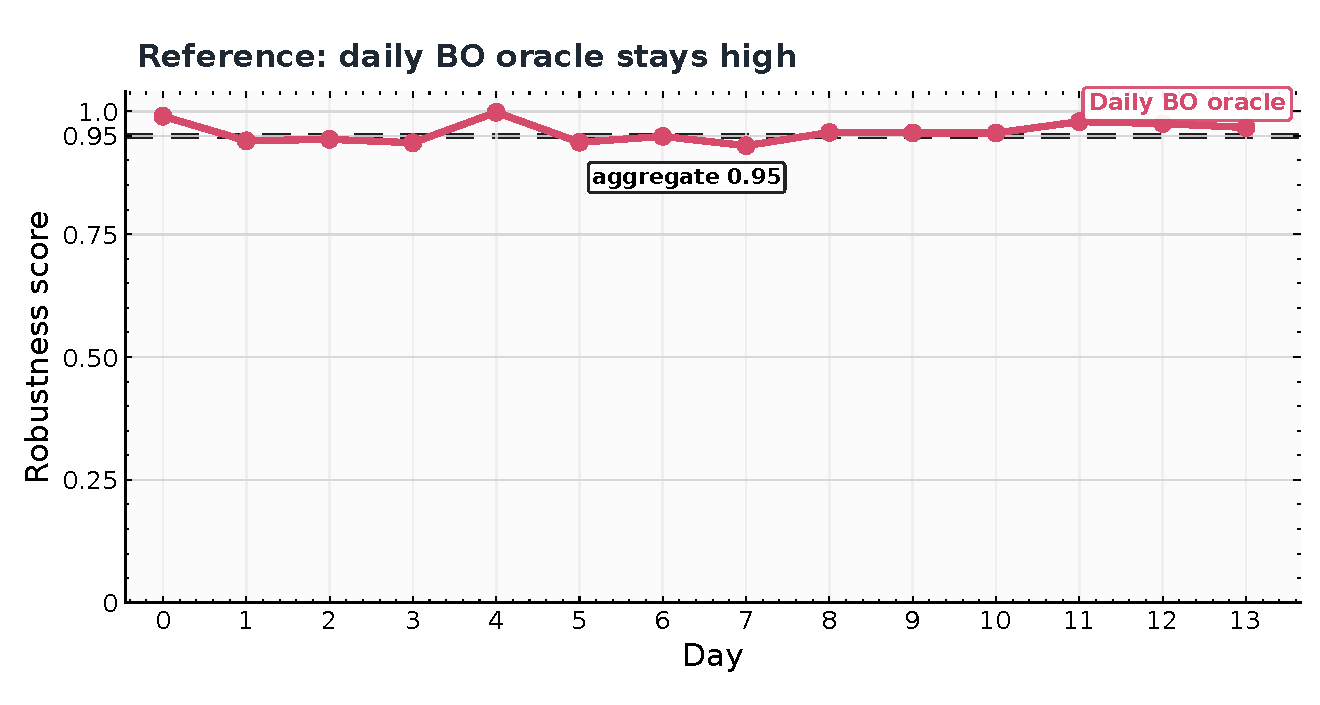
\includegraphics[width=\linewidth,height=0.71\textheight,keepaspectratio]{figures/results/main_results_overlays/main_results_overlay_1.pdf}}
        \only<2>{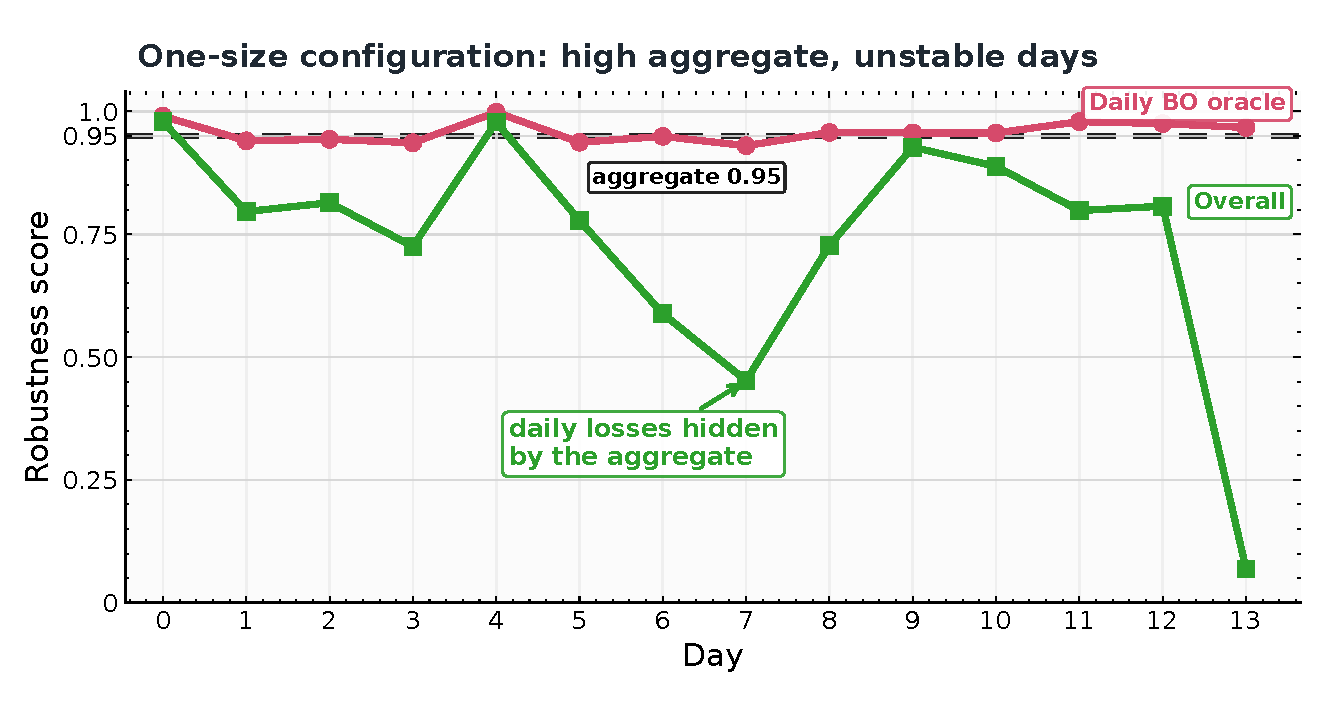
\includegraphics[width=\linewidth,height=0.71\textheight,keepaspectratio]{figures/results/main_results_overlays/main_results_overlay_2.pdf}}
        \only<3>{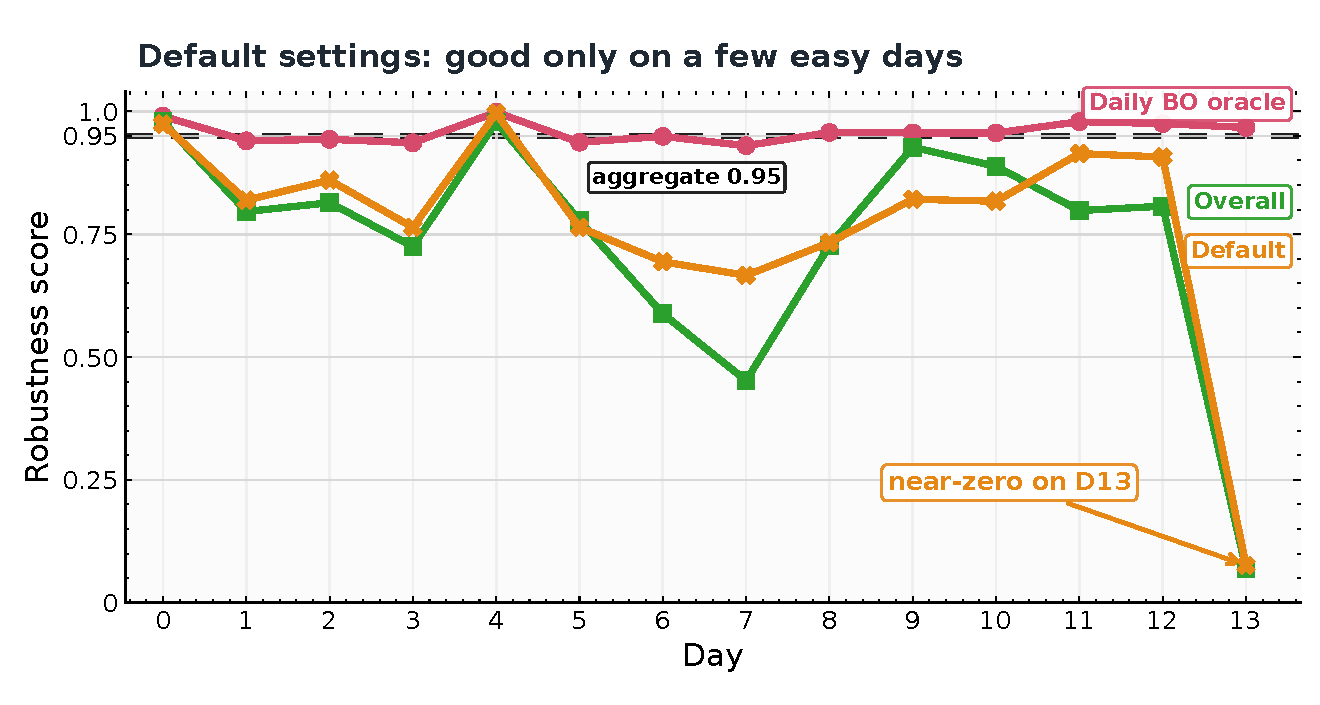
\includegraphics[width=\linewidth,height=0.71\textheight,keepaspectratio]{figures/results/main_results_overlays/main_results_overlay_3.pdf}}
        \only<4>{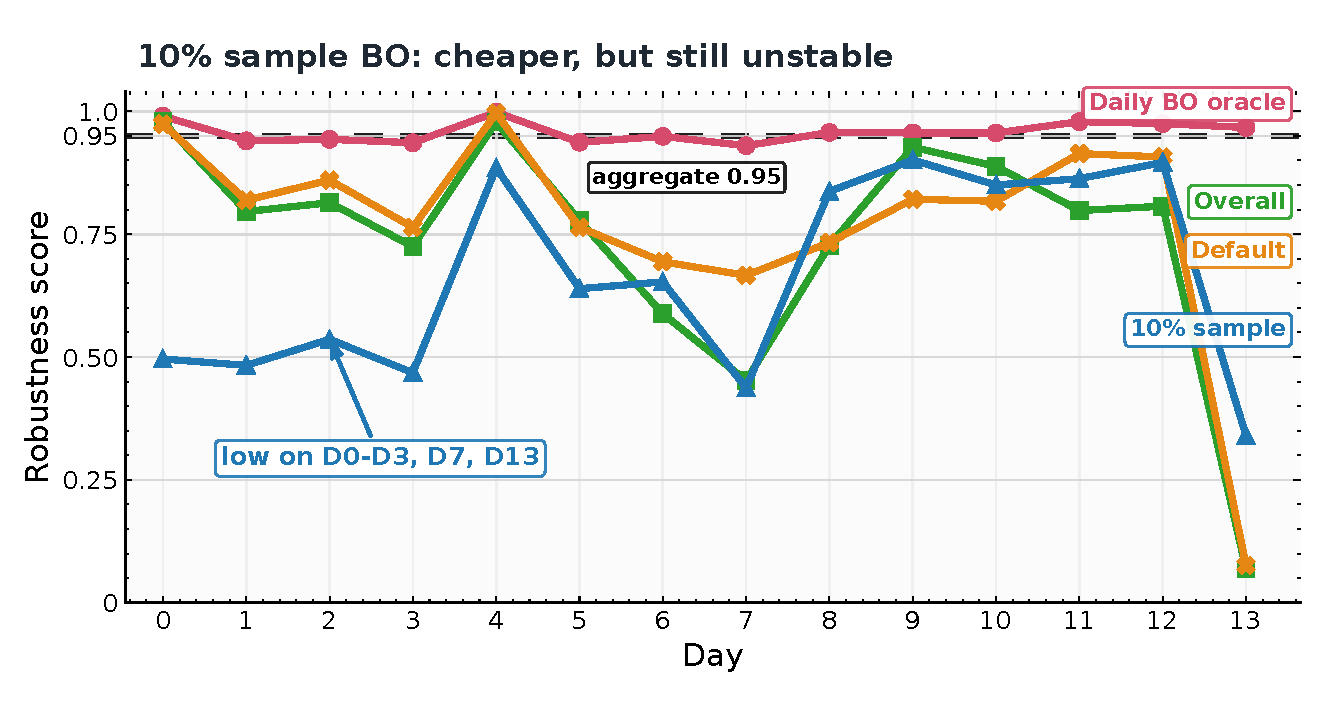
\includegraphics[width=\linewidth,height=0.71\textheight,keepaspectratio]{figures/results/main_results_overlays/main_results_overlay_4.pdf}}
        \only<5>{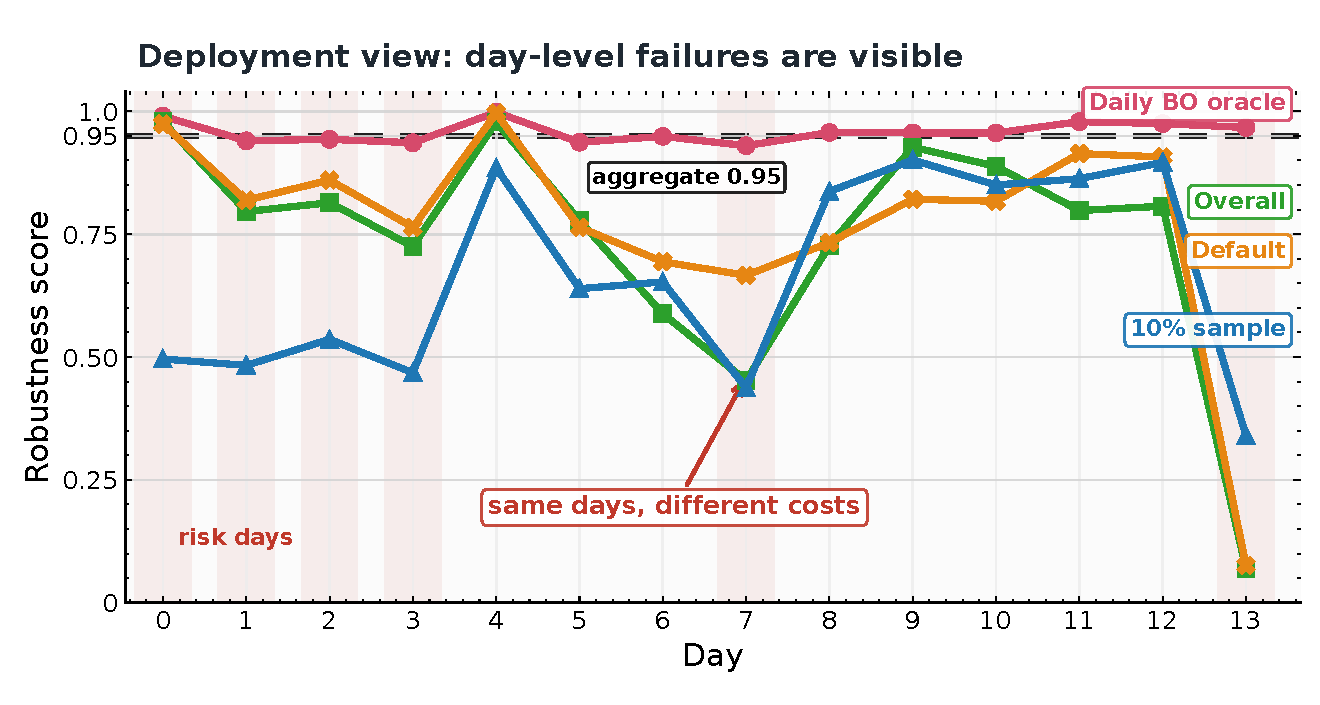
\includegraphics[width=\linewidth,height=0.71\textheight,keepaspectratio]{figures/results/main_results_overlays/main_results_overlay_5.pdf}}

        \vspace{0.15em}
        {\scriptsize\color{black!70}Daily robustness across configuration strategies}
    \end{columns}

    \vfill
    \centering
    \visible<5->{\color{structure.fg}\small
        \(\Longrightarrow\) Low-budget configurations do not reliably approximate the daily BO oracle.}
\end{frame}

\begin{frame}[plain]
    \centering
    \vfill
    {\color{structure.fg}\Large\bfseries Research Question 2}

    \vspace{1.2em}
    \begin{minipage}{0.88\linewidth}
        \centering
        {\LARGE\bfseries If \(\theta\) is reused,\par}
        \vspace{0.25em}
        {\LARGE\bfseries how much performance is lost\par}
        \vspace{0.25em}
        {\LARGE\bfseries compared with reconfiguring\par}
        \vspace{0.25em}
        {\LARGE\bfseries for the current network context?\par}
    \end{minipage}
    \vfill
\end{frame}

\begin{frame}{Day-to-Day Transferability: Method}
    \vspace{-0.35em}
    \begin{columns}[T,onlytextwidth]
        \column{0.43\linewidth}
        \scriptsize
        \begin{itemize}
            \setlength\itemsep{0.45em}
            \item<1-> BO gives one oracle configuration per day; pick a source \(D_j\) with \(\theta_j^{\star}\).
            \item<2-> Diagonal cells are oracle references, not transfer evaluations.
            \item<3-> Keep \(\theta_j^{\star}\) fixed and evaluate it on every target day \(D_i\), excluding \(i=j\).
            \item<4-> Repeating this for all source days fills the off-diagonal matrix.
            \item<5-> Example: \(R_0\) collects all transfer losses for target day \(D_0\) and becomes one box plot.
        \end{itemize}

        \vfill
        \visible<5->{\color{structure.fg}\footnotesize
            \(\Longrightarrow\) Lower row losses indicate safer configuration reuse.}

        \column{0.55\linewidth}
        \centering
        \resizebox{\linewidth}{!}{%
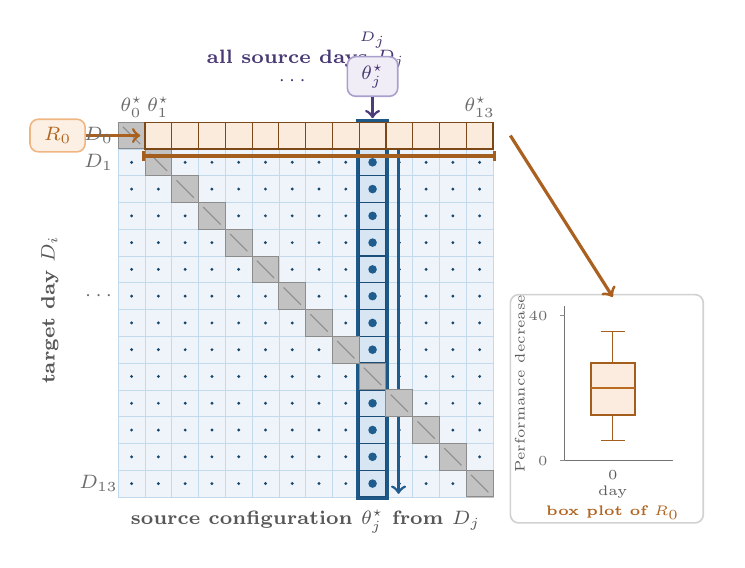
\begin{tikzpicture}[font=\sffamily\scriptsize,line width=0.58pt]
    \definecolor{dayblue}{RGB}{42,122,188}
    \definecolor{configviolet}{RGB}{103,80,164}
    \definecolor{riskorange}{RGB}{227,130,42}
    \definecolor{safegreen}{RGB}{42,150,95}

    \tikzset{
        arrow/.style={->,draw=#1!75!black,line width=1.0pt},
        every node/.style={text=black!82}
    }

    \path[use as bounding box] (0,0) rectangle (8.75,6.50);

    \def\mx{1.15}
    \def\my{5.30}
    \def\s{0.34}
    \def\targetrow{0}
    \def\sourcecol{9}

    \pgfmathsetmacro{\ytop}{\my-\targetrow*\s}
    \pgfmathsetmacro{\ycenter}{\my-\targetrow*\s-0.5*\s}
    \pgfmathsetmacro{\xsource}{\mx+\sourcecol*\s}
    \pgfmathsetmacro{\xcenter}{\mx+\sourcecol*\s+0.5*\s}

    % Base matrix.
    \foreach \r in {0,...,13}{
        \foreach \c in {0,...,13}{
            \pgfmathsetmacro{\x}{\mx+\c*\s}
            \pgfmathsetmacro{\y}{\my-\r*\s}
            \draw[draw=black!24,fill=white,line width=0.30pt] (\x,\y) rectangle ++(\s,-\s);
        }
    }

    % Step 4: repeating over all source configurations fills the off-diagonal matrix.
    \visible<4->{
        \foreach \r in {0,...,13}{
            \foreach \c in {0,...,13}{
                \ifnum\r=\c\relax
                \else
                    \pgfmathsetmacro{\x}{\mx+\c*\s}
                    \pgfmathsetmacro{\y}{\my-\r*\s}
                    \pgfmathsetmacro{\xc}{\mx+\c*\s+0.5*\s}
                    \pgfmathsetmacro{\yc}{\my-\r*\s-0.5*\s}
                    \draw[draw=dayblue!28,fill=dayblue!8,line width=0.25pt] (\x,\y) rectangle ++(\s,-\s);
                    \fill[dayblue!58!black] (\xc,\yc) circle (0.58pt);
                \fi
            }
        }
        \node[font=\bfseries\scriptsize,text=configviolet!70!black] at ({\mx+7*\s},6.10) {all source days \(D_j\)};
        \pgfmathsetmacro{\xellipsis}{\mx+6*\s+0.5*\s}
        \node[font=\scriptsize,text=configviolet!70!black] at (\xellipsis,5.82) {$\cdots$};
    }

    % Step 1: pick one source configuration column.
    \visible<1-3>{
        \foreach \r in {0,...,13}{
            \pgfmathsetmacro{\y}{\my-\r*\s}
            \draw[draw=configviolet!42,fill=configviolet!10,line width=0.34pt] (\xsource,\y) rectangle ++(\s,-\s);
        }
        \node[draw=configviolet!55,fill=configviolet!10,rounded corners=3pt,inner xsep=5pt,inner ysep=3pt,font=\bfseries\scriptsize,text=configviolet!70!black]
            (sourcecfg) at (\xcenter,5.88) {$\theta_j^{\star}$};
        \node[font=\tiny,text=configviolet!65!black] at (\xcenter,6.34) {$D_j$};
        \draw[arrow=configviolet] (sourcecfg.south) -- (\xcenter,{\my+0.05});
    }

    % Step 3: keep that configuration fixed and test it down the full target-day column.
    \visible<3>{
        \foreach \r in {0,...,13}{
            \pgfmathsetmacro{\y}{\my-\r*\s}
            \pgfmathsetmacro{\yc}{\my-\r*\s-0.5*\s}
            \draw[draw=dayblue!64!black,fill=dayblue!19,line width=0.46pt] (\xsource,\y) rectangle ++(\s,-\s);
            \fill[dayblue!76!black] (\xcenter,\yc) circle (1.55pt);
        }
        \draw[draw=dayblue!72!black,line width=1.05pt]
            ({\xsource-0.025},{\my+0.02}) rectangle ({\xsource+\s+0.025},{\my-14*\s-0.02});
        \draw[arrow=dayblue] ({\xsource+\s+0.16},{\my-0.03}) -- ({\xsource+\s+0.16},{\my-14*\s+0.04});
    }

    % Step 2: oracle diagonal excluded from transfer.
    \visible<2->{
        \foreach \d in {0,...,13}{
            \pgfmathsetmacro{\x}{\mx+\d*\s}
            \pgfmathsetmacro{\y}{\my-\d*\s}
            \draw[draw=black!45,fill=black!24,line width=0.35pt] (\x,\y) rectangle ++(\s,-\s);
            \draw[draw=black!45,line width=0.35pt] (\x+0.060,\y-0.060) -- (\x+\s-0.060,\y-\s+0.060);
        }
    }

    % Step 5: read one target row as a distribution / box plot.
    \visible<5->{
        \foreach \c in {1,...,13}{
            \pgfmathsetmacro{\x}{\mx+\c*\s}
            \draw[draw=riskorange!55!black,fill=riskorange!16,line width=0.42pt] (\x,\ytop) rectangle ++(\s,-\s);
        }
        \node[draw=riskorange!58,fill=riskorange!12,rounded corners=3pt,inner xsep=5pt,inner ysep=3pt,font=\bfseries\scriptsize,text=riskorange!78!black]
            (rowdist) at (0.38,\ycenter) {$R_0$};
        \draw[arrow=riskorange] (rowdist.east) -- ({\mx+\s-0.06},\ycenter);

        \draw[draw=riskorange!72!black,line width=1.1pt]
            ({\mx+\s-0.02},{\ytop-\s-0.09}) -- ({\mx+14*\s+0.02},{\ytop-\s-0.09});
        \draw[draw=riskorange!72!black,line width=1.1pt]
            ({\mx+\s-0.02},{\ytop-\s-0.03}) -- ({\mx+\s-0.02},{\ytop-\s-0.15});
        \draw[draw=riskorange!72!black,line width=1.1pt]
            ({\mx+14*\s+0.02},{\ytop-\s-0.03}) -- ({\mx+14*\s+0.02},{\ytop-\s-0.15});
        % Chart-style preview of the final box-plot result.
        \node[draw=black!18,fill=white,rounded corners=3pt,minimum width=2.45cm,minimum height=2.90cm,anchor=south west] at (6.12,0.20) {};
        \draw[draw=black!55,line width=0.45pt] (6.82,1.00) -- (8.20,1.00);
        \draw[draw=black!55,line width=0.45pt] (6.82,1.00) -- (6.82,2.96);
        \node[font=\tiny,text=black!64] at (7.43,0.82) {0};
        \node[font=\tiny,text=black!64] at (7.43,0.60) {day};
        \node[font=\tiny,text=black!64,rotate=90] at (6.25,1.98) {Performance decrease};
        \foreach \y/\lab in {1.00/0,2.84/40}{
            \draw[draw=black!45,line width=0.35pt] (6.76,\y) -- (6.82,\y);
            \node[font=\tiny,text=black!58,anchor=east] at (6.73,\y) {\lab};
        }
        \draw[draw=riskorange!72!black,line width=0.55pt] (7.43,1.26) -- (7.43,2.64);
        \draw[draw=riskorange!72!black,line width=0.55pt] (7.28,1.26) -- (7.58,1.26);
        \draw[draw=riskorange!72!black,line width=0.55pt] (7.28,2.64) -- (7.58,2.64);
        \draw[draw=riskorange!72!black,fill=riskorange!15,line width=0.65pt] (7.15,1.58) rectangle (7.71,2.24);
        \draw[draw=riskorange!82!black,line width=0.75pt] (7.15,1.92) -- (7.71,1.92);
        \node[font=\bfseries\tiny,text=riskorange!78!black] at (7.43,0.34) {box plot of $R_0$};
        \draw[arrow=riskorange,line width=1.15pt] ({\mx+14*\s+0.22},\ycenter) -- (7.43,3.08);
    }

    % Sparse numeric anchors after overlays so they remain readable.
    \foreach \c/\lab in {0/$\theta_0^{\star}$,1/$\theta_1^{\star}$,13/$\theta_{13}^{\star}$}{
        \pgfmathsetmacro{\x}{\mx+\c*\s+0.5*\s}
        \node[font=\scriptsize,text=black!58] at (\x,5.49) {\lab};
    }
    \foreach \r/\lab in {0/$D_0$,1/$D_1$,6/$\cdots$,13/$D_{13}$}{
        \pgfmathsetmacro{\y}{\my-\r*\s-0.5*\s}
        \node[font=\scriptsize,text=black!58] at (0.90,\y) {\lab};
    }

    \node[font=\bfseries\scriptsize,text=black!66]
        at ({\mx+7*\s},0.23) {source configuration $\theta_j^{\star}$ from $D_j$};
    \node[font=\bfseries\scriptsize,text=black!66,rotate=90]
        at (0.28,{\my-7*\s}) {target day $D_i$};
\end{tikzpicture}%
}

    \end{columns}
\end{frame}

\begin{frame}{Day-to-Day Transferability: Results}
    \scriptsize
    \begin{columns}[T,onlytextwidth]
        \column{0.38\linewidth}
        \begin{itemize}
            \setlength\itemsep{0.45em}
            \item Each box summarizes one target day
                  \(R_i=\{\Delta(i,j): j\neq i\}\).
            \item Low medians indicate small transfer loss for most source configurations.
            \item Wide boxes and outliers show sensitivity to the chosen source day.
            \item Days 5--7 and 10 are the riskiest; losses can approach 40\%.
        \end{itemize}

        \vfill
        {\color{structure.fg}\footnotesize
            \(\Longrightarrow\) Transferability is day-dependent, not universal.}

        \column{0.59\linewidth}
        \centering
        \includegraphics[height=0.70\textheight,keepaspectratio]{/home/oanser/Documents/work/noms2026/sections/figures/transferability_box_plot.pdf}

        \vspace{0.15em}
        {\scriptsize\color{black!70}Transfer loss distributions by target day}
    \end{columns}
\end{frame}

\begin{frame}{Cross-Year Attack Transfer: Method}
    \vspace{-0.35em}
    \begin{columns}[T,onlytextwidth]
        \column{0.40\linewidth}
        \scriptsize
        \begin{itemize}
            \setlength\itemsep{0.45em}
            \item<1-> Select one of the 18 attack families common to IDS2017 and IDS2018.
            \item<2-> Build paired datasets for the same attack \(a_k\) in both years.
            \item<3-> BO gives \(\theta^{\star\,2017}_{a_k}\) and the IDS2018 oracle \(\theta^{\star\,2018}_{a_k}\).
            \item<4-> Evaluate both configurations on \(\mathcal{D}^{2018}_{a_k}\) and measure the gap.
        \end{itemize}

        \vfill
        \visible<4->{\color{structure.fg}\footnotesize
            \(\Longrightarrow\) Same attack does not imply same robust configuration.}

        \column{0.58\linewidth}
        \centering
        \resizebox{\linewidth}{!}{%
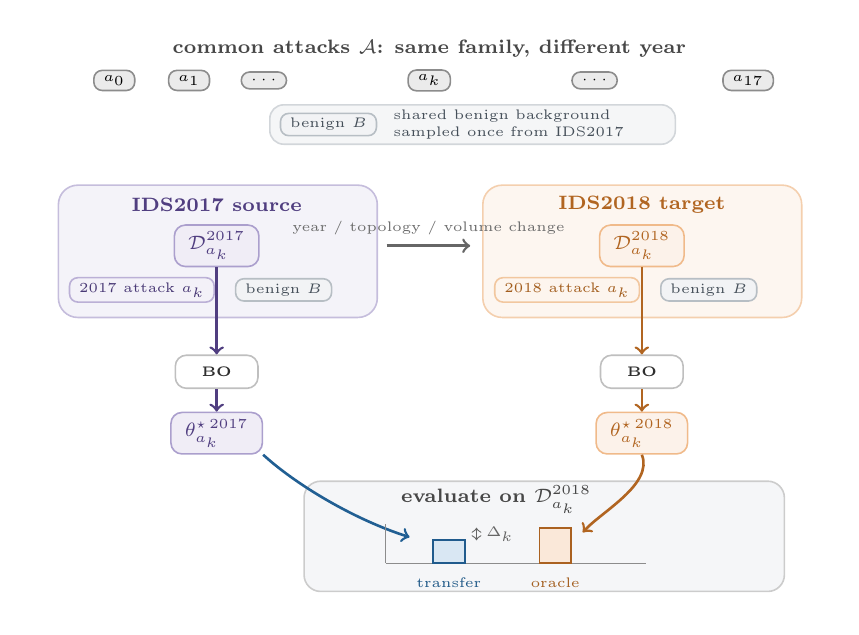
\begin{tikzpicture}[font=\sffamily\scriptsize,line width=0.58pt]
    \definecolor{sourceviolet}{RGB}{103,80,164}
    \definecolor{targetorange}{RGB}{227,130,42}
    \definecolor{transferblue}{RGB}{42,122,188}
    \definecolor{benigngray}{RGB}{96,110,124}
    \definecolor{softgray}{RGB}{245,246,248}

    \tikzset{
        panel/.style={rounded corners=7pt,draw=#1!38,fill=#1!7,inner sep=0pt},
        chip/.style={rounded corners=4pt,draw=#1!55,fill=#1!10,inner xsep=5pt,inner ysep=2.5pt,font=\bfseries\scriptsize,text=#1!78!black},
        smallchip/.style={rounded corners=3pt,draw=#1!45,fill=#1!8,inner xsep=3.5pt,inner ysep=1.8pt,font=\tiny,text=#1!72!black},
        arrow/.style={->,draw=#1!78!black,line width=0.95pt},
        every node/.style={text=black!82}
    }

    \path[use as bounding box] (0,0) rectangle (10.20,7.35);

    % Step 1: choose one attack common to both years and the shared benign background.
    \visible<1->{
        \node[font=\bfseries\scriptsize,text=black!72] at (5.10,7.08)
            {common attacks \(\mathcal{A}\): same family, different year};
        \foreach \x/\lab in {1.10/$a_0$,2.05/$a_1$,3.00/$\cdots$,7.20/$\cdots$,9.15/$a_{17}$}{
            \node[smallchip=black] at (\x,6.68) {\lab};
        }
        \node[smallchip=black] at (5.10,6.68) {$a_k$};

        \node[draw=benigngray!28,fill=benigngray!6,rounded corners=5pt,minimum width=5.15cm,minimum height=0.50cm]
            at (5.65,6.12) {};
        \node[smallchip=benigngray] at (3.82,6.12) {benign \(B\)};
        \node[align=left,font=\tiny,text=benigngray!72!black,anchor=west]
            at (4.52,6.12) {shared benign background\\sampled once from IDS2017};
    }

    % Step 2: build paired datasets for the selected attack.
    \visible<2->{
        \node[panel=sourceviolet,minimum width=4.05cm,minimum height=1.68cm,anchor=north west] at (0.38,5.36) {};
        \node[panel=targetorange,minimum width=4.05cm,minimum height=1.68cm,anchor=north west] at (5.77,5.36) {};

        \node[font=\bfseries\scriptsize,text=sourceviolet!78!black] at (2.40,5.10) {IDS2017 source};
        \node[font=\bfseries\scriptsize,text=targetorange!78!black] at (7.80,5.10) {IDS2018 target};

        \node[chip=sourceviolet] (d17) at (2.40,4.58) {$\mathcal{D}^{2017}_{a_k}$};
        \node[chip=targetorange] (d18) at (7.80,4.58) {$\mathcal{D}^{2018}_{a_k}$};

        \node[smallchip=sourceviolet] at (1.45,4.02) {2017 attack \(a_k\)};
        \node[smallchip=benigngray] (b17) at (3.25,4.02) {benign \(B\)};
        \node[smallchip=targetorange] at (6.85,4.02) {2018 attack \(a_k\)};
        \node[smallchip=benigngray] (b18) at (8.65,4.02) {benign \(B\)};

        \draw[->,draw=black!60,line width=0.95pt] (4.56,4.58) -- node[above,font=\tiny,text=black!58] {year / topology / volume change} (5.62,4.58);
    }

    % Step 3: optimize both year-specific datasets.
    \visible<3->{
        \node[draw=black!25,fill=white,rounded corners=4pt,minimum width=1.05cm,minimum height=0.42cm,font=\bfseries\tiny] (bo17) at (2.40,2.98) {BO};
        \node[draw=black!25,fill=white,rounded corners=4pt,minimum width=1.05cm,minimum height=0.42cm,font=\bfseries\tiny] (bo18) at (7.80,2.98) {BO};
        \draw[arrow=sourceviolet] (d17.south) -- (bo17.north);
        \draw[arrow=targetorange] (d18.south) -- (bo18.north);

        \node[chip=sourceviolet] (theta17) at (2.40,2.20) {$\theta^{\star\,2017}_{a_k}$};
        \node[chip=targetorange] (theta18) at (7.80,2.20) {$\theta^{\star\,2018}_{a_k}$};
        \draw[arrow=sourceviolet] (bo17.south) -- (theta17.north);
        \draw[arrow=targetorange] (bo18.south) -- (theta18.north);
    }

    % Step 4: evaluate both configurations on IDS2018 and compare.
    \visible<4->{
        \node[draw=black!20,fill=softgray,rounded corners=6pt,minimum width=6.10cm,minimum height=1.40cm,anchor=south west] at (3.50,0.18) {};
        \node[font=\bfseries\scriptsize,text=black!72] at (5.95,1.36) {evaluate on \(\mathcal{D}^{2018}_{a_k}\)};

        \draw[arrow=transferblue] (theta17.south east) .. controls (3.40,1.55) and (4.15,1.10) .. (4.85,0.88);
        \draw[arrow=targetorange] (theta18.south) .. controls (7.95,1.55) and (7.28,1.20) .. (7.05,0.94);

        \draw[draw=black!45,line width=0.35pt] (4.55,0.55) -- (7.85,0.55);
        \draw[draw=black!45,line width=0.35pt] (4.55,0.55) -- (4.55,1.05);
        \draw[draw=transferblue!75!black,fill=transferblue!18,line width=0.65pt] (5.15,0.55) rectangle (5.55,0.84);
        \draw[draw=targetorange!75!black,fill=targetorange!18,line width=0.65pt] (6.50,0.55) rectangle (6.90,1.00);
        \node[font=\tiny,text=transferblue!72!black] at (5.35,0.30) {transfer};
        \node[font=\tiny,text=targetorange!72!black] at (6.70,0.30) {oracle};
        \draw[<->,draw=black!60,line width=0.40pt] (5.70,0.84) -- node[right,font=\tiny,text=black!60] {$\Delta_k$} (5.70,1.00);
    }
\end{tikzpicture}%
}

    \end{columns}
\end{frame}

\begin{frame}{Cross-Year Attack Transfer: Results}
    \scriptsize
    \begin{columns}[T,onlytextwidth]
        \column{0.38\linewidth}
        \begin{itemize}
            \setlength\itemsep{0.45em}
            \item Each attack family compares IDS2017-tuned transfer against the IDS2018 oracle.
            \item Attacks 23, 17, 16, 14, and 26 transfer close to the oracle.
            \item Attacks 31, 1, and 30 show much larger cross-year gaps.
            \item Same attack family is therefore not enough to guarantee robust reuse.
        \end{itemize}

        \vfill
        {\color{structure.fg}\footnotesize
            \(\Longrightarrow\) Cross-year context changes can still require reconfiguration.}

        \column{0.59\linewidth}
        \centering
        \includegraphics[width=\linewidth,height=0.68\textheight,keepaspectratio]{/home/oanser/Documents/work/noms2026/sections/figures/attacks_transfer_IDS2017_to_IDS2018.pdf}

        \vspace{0.15em}
        {\scriptsize\color{black!70}IDS2017 configuration transferred to IDS2018 by attack family}
    \end{columns}
\end{frame}
